% Author: Milos A. Saric, copyright 2025. https://saricmilos.com/

\title{Book Recommendation System --- Collaborative, Content-Based \& Hybrid Filtering Approaches}
\date{\today}
\author{Milos Saric}
\maketitle



% --------------- ABSTRACT
\begin{abstract}
This report investigates the Kaggle Book Recommendation dataset to develop intelligent book recommendation systems using both
collaborative filtering and content-based methods. A key application of machine learning is generating personalized recommendations
for users, aiming to boost revenue, engagement, or other performance metrics. As a result, understanding how these recommendation
algorithms work is an essential skill for any Machine Learning Engineer.
Recommender systems have become a vital component of online platforms such
as YouTube, Amazon, and Netflix, helping users discover content tailored to their preferences. By analyzing user behavior and
item attributes, these systems predict user interests, enhancing user experience while driving engagement and revenue. 
This study highlights the implementation, advantages, and practical significance of recommendation algorithms in modern
digital platforms.
\end{abstract}

\rule{\linewidth}{0.5pt}

\section{Introduction and Problem Definition}

Recommender systems aim to predict user preferences and suggest items they are most likely to enjoy. 
This project focuses on developing a \textbf{book recommendation system} using the Kaggle \textbf{Book-Crossing Dataset},
leveraging both \textbf{collaborative}, \textbf{content-based approaches} and \textbf{hybrid filtering approaches} to deliver personalized
book suggestions.
The goal is to design a system that accurately predicts and recommends books a user is likely to enjoy based on past interactions,
ratings, and preferences. A clear understanding of this problem ensures that all subsequent analysis and modeling efforts align
with the primary objective.

The main purpose of a recommender system is to boost product sales. Businesses use these systems to maximize their profits by
suggesting products that customers are likely to be interested in. By highlighting relevant and appealing items, recommender
systems help users discover products they might otherwise miss — ultimately driving higher sales and greater profits for the company.

\begin{center}
\begin{tikzpicture}[node distance=2cm,
    rec/.style={rectangle, draw=black, fill=#1!40, rounded corners, minimum width=3.5cm, minimum height=1cm, align=center, font=\small},
    arrow/.style={-{Stealth}, thick},
    every node/.style={font=\small}
]

    % Nodes with colors
    \node[rec=orange] (RS) {Recommender Systems};
    \node[rec=cyan] (CF) [below left of=RS, xshift=-3cm] {Collaborative Filtering};
    \node[rec=green] (CB) [below of=RS] {Content-Based Filtering};
    \node[rec=purple] (Hybrid) [below right of=RS, xshift=3cm] {Hybrid Filtering};
    \node[rec=blue] (User) [below left of=CF, xshift=-1.5cm, yshift=-0.5cm] {User-Based};
    \node[rec=red] (Item) [below right of=CF, xshift=1.5cm, yshift=-0.5cm] {Item-Based};

    % Arrows
    \draw[arrow] (RS) -- (CF);
    \draw[arrow] (RS) -- (CB);
    \draw[arrow] (RS) -- (Hybrid);
    \draw[arrow] (CF) -- (User);
    \draw[arrow] (CF) -- (Item);
\end{tikzpicture}
\end{center}

\subsection{Scope}
The analysis focuses exclusively on the Kaggle dataset, which includes:  
\begin{itemize}
    \item \textbf{Users:} demographic and identification data.  
    \item \textbf{Books:} metadata such as title, author, year, publisher, and cover images.  
    \item \textbf{Ratings:} explicit ratings (1--10) and implicit feedback (0 for interactions without ratings).  
\end{itemize}
Predictions are restricted to this dataset without using external sources unless explicitly integrated in advanced phases.

\subsection{Stakeholders}
\begin{itemize}
    \item \textbf{Readers / Users:} receive personalized book recommendations.  
    \item \textbf{Publishers / Authors:} gain insights into reader interests for better targeting.  
    \item \textbf{Data Scientists / ML Practitioners:} test and optimize recommendation algorithms.  
    \item \textbf{Platform Developers / Businesses:} improve user engagement, retention, and revenue through effective recommendations.
\end{itemize}


\section{Neighborhood-Based Collaborative Filtering}

Collaborative filtering creates a model based on a user's past actions such as items they have purchased, selected, or
rated, as well as the behavior of other users with similar preferences. This model is then used to recommend items or predict 
ratings for items that the user is likely to be interested in.
Collaborative filtering is a recommendation method that predicts a users preferences based on the choices of other users
with similar tastes. It relies on both user and item information, often organized in a user-item matrix.

This approach is widely used in industry across platforms like YouTube, Netflix and Amazon. 
For example, if users with similar past actions/tastes buy a product on Amazon, the system can suggest that same product to you.
YouTube leverages this technique to recommend videos, Amazon uses it to suggest books and products, and Netflix relies heavily on
collaborative filtering to personalize movie recommendations.

\begin{center}
\begin{tikzpicture}[
    user/.style={rectangle, draw=black, fill=cyan!25, rounded corners, minimum width=2.6cm, minimum height=0.9cm, align=center, font=\small},
    item/.style={rectangle, draw=black, fill=green!20, rounded corners, minimum width=2.6cm, minimum height=0.9cm, align=center, font=\small},
    like/.style={-{Stealth}, thick},
    recommend/.style={-{Stealth}, thick, dashed, red},
    similar/.style={<->, very thick, purple!70},
    every node/.style={font=\small}
]

    % Users
    \node[user] (User1) {User 1};
    \node[user] (User2) [right=6.0cm of User1] {User 2};

    % Similarity label and arrow between users
    \draw[similar] (User1) -- node[above=3pt]{\footnotesize similar} (User2);

    % Books for User1 (spaced out horizontally)
    \node[item] (Book1) [below=3.0cm of User1, xshift=-2.0cm] {1984};
    \node[item] (Book2) [below=3.0cm of User1, xshift= 2.0cm] {Steve Jobs};

    % Books for User2 (spaced out horizontally, wider spacing)
    \node[item] (Book3) [below=3.0cm of User2, xshift=-3.0cm] {1984};
    \node[item] (Book4) [below=3.0cm of User2, xshift= 0.0cm] {Steve Jobs};
    \node[item] (Book5) [below=3.0cm of User2, xshift= 3.0cm] {Stiff};

    % Arrows from User1 to books (solid)
    \draw[like] (User1.south) -- (Book1.north);
    \draw[like] (User1.south) -- (Book2.north);

    % Arrows from User2 to books (solid)
    \draw[like] (User2.south) -- (Book3.north);
    \draw[like] (User2.south) -- (Book4.north);
    \draw[like] (User2.south) -- (Book5.north);

    % Recommendation arrow from Book5 to User1 with label above the line
    \draw[recommend] (Book5.north) to[out=90,in=40] node[midway, above]{\footnotesize recommend} (User1.south);

    % Legend (top-left)
    \node[draw=none, fill=none, above=1.1cm of User1, align=left] (legend) {
      \begin{tabular}{@{}ll@{}}
        \raisebox{0.5ex}{\tikz{\draw[like] (0,0)--(0.6,0);}} & like \\
        \raisebox{0.5ex}{\tikz{\draw[recommend] (0,0)--(0.6,0);}} & recommend \\
        \raisebox{0.5ex}{\tikz{\draw[similar] (0,0)--(0.6,0);}} & similar
      \end{tabular}
    };

\end{tikzpicture}
\end{center}

\begin{center}
\resizebox{\textwidth}{!}{%
\begin{tikzpicture}[every node/.style={transform shape},
    user/.style={rectangle, draw=black, fill=cyan!25, rounded corners, minimum width=2.2cm, minimum height=0.9cm, align=center, font=\small},
    item/.style={rectangle, draw=black, fill=green!18, rounded corners, minimum width=2.2cm, minimum height=0.9cm, align=center, font=\small},
    like/.style={-{Stealth}, thick},
    recommend/.style={-{Stealth}, thick, dashed, red},
    similar/.style={<->, very thick, purple!60}
]

%%%%% Use symmetric xshifts so left and right diagrams are identical in size
\begin{scope}[xshift=-6.5cm]  % left diagram (negative shift)
    % Users (vertical)
    \node[user] (A) {User A};
    \node[user, below=0.9cm of A] (B) {User B};
    \node[user, below=0.9cm of B] (C) {User C};

    % Items (to the right of users), spaced to avoid overlap
    \node[item, right=3.6cm of A] (IA) {Book A};
    \node[item, below=1.1cm of IA] (IB) {Book B};
    \node[item, below=1.1cm of IB] (IC) {Book C};
    \node[item, below=1.1cm of IC] (ID) {Book D};

    % Similarity label & arrow (left side connecting A and C)
    \draw[-{Stealth}, thick] ($(A.west)+(-0.6,0)$) -- ($(C.west)+(-0.6,0)$) node[midway,left]{\footnotesize similar};

    % Like arrows
    \draw[like] (A) -- (IA);
    \draw[like] (A) -- (IC);
    \draw[like] (B) -- (IB);
    \draw[like] (C) -- (IA);
    \draw[like] (C) -- (IC);
    \draw[like] (C) -- (ID);

    % Recommend arrow (dashed red) from ID to A with label above
    \draw[recommend] (ID.north) to[out=85,in=0] node[midway, above]{\footnotesize recommend} (A.south);

    % Legend
    \node[draw=none, fill=none, above=0.9cm of A, align=left] (legendL) {
      \begin{tabular}{@{}ll@{}}
        \raisebox{0.5ex}{\tikz{\draw[like] (0,0)--(0.6,0);}} & like \\
        \raisebox{0.5ex}{\tikz{\draw[recommend] (0,0)--(0.6,0);}} & recommend \\
        \raisebox{0.5ex}{\tikz{\draw[similar] (0,0)--(0.6,0);}} & similar
      \end{tabular}
    };

    % Caption
    \node[below=1.2cm of C] {\textbf{User-Based CF}};
\end{scope}

\begin{scope}[xshift=+6.5cm]  % right diagram (positive shift)
    % Users (vertical)
    \node[user] (U1) {User A};
    \node[user, below=0.9cm of U1] (U2) {User B};
    \node[user, below=0.9cm of U2] (U3) {User C};

    % Items (to the right of users) — same spacing as left
    \node[item, right=3.6cm of U1] (IA2) {Book A};
    \node[item, below=1.1cm of IA2] (IB2) {Book B};
    \node[item, below=1.1cm of IB2] (IC2) {Book C};
    \node[item, below=1.1cm of IC2] (ID2) {Book D};

    % Like arrows (solid)
    \draw[like] (U1) -- (IA2);
    \draw[like] (U1) -- (IC2);
    \draw[like] (U1) -- (ID2);
    \draw[like] (U2) -- (IA2);
    \draw[like] (U2) -- (ID2);
    \draw[like] (U3) -- (IA2);

    % Recommend arrow from ID2 to U3 with label above the line
    \draw[recommend] (ID2.north) to[out=85,in=20] node[midway, above]{\footnotesize recommend} (U3.south);

    % Similarity between items (right side) — arrow & label
    \draw[-{Stealth}, thick] (IA2.east) -- ++(0.9,-2.8) node[midway,right]{\footnotesize similar};
    \draw[like] (ID2.east) -- ++(0.9,2.8);

    % Legend
    \node[draw=none, fill=none, above=0.9cm of U1, align=left] (legendR) {
      \begin{tabular}{@{}ll@{}}
        \raisebox{0.5ex}{\tikz{\draw[like] (0,0)--(0.6,0);}} & like \\
        \raisebox{0.5ex}{\tikz{\draw[recommend] (0,0)--(0.6,0);}} & recommend
      \end{tabular}
    };

    % Caption
    \node[below=1.2cm of U3] {\textbf{Item-Based CF}};
\end{scope}

\end{tikzpicture}%
} % end resizebox
\end{center}

Collaborative filtering relies heavily on user data. As users continue to browse, purchase, and rate products, their preferences evolve over time. Because of this, the underlying recommendation model must be regularly updated and refined to stay accurate and relevant. In practice, this means continuously integrating new data and adjusting the system to reflect changing user behavior and market trends.

The two main sources of data for collaborative filtering are:

\begin{itemize}
    \item \textbf{Explicit data:} Information that users actively provide, such as ratings, reviews, or responses to surveys and questionnaires.
    \item \textbf{Implicit data:} Information inferred from user behavior, including browsing history, clicks, time spent on content, likes, shares, and other engagement signals.
\end{itemize}

Both types of data are essential for understanding user preferences. Explicit ratings capture direct feedback, while implicit data reveals natural behavioral patterns that help improve recommendation accuracy over time.

\subsection{User-Based Collaborative Filtering}
User-based collaborative filtering recommends items to a user by identifying other users with similar preferences. 
If a similar user liked an item, it can be suggested. 
In our user based book recommendation system, we begin by constructing a matrix with users as rows and books (identified by ISBN) 
as columns let's call this the user-book matrix.

Each entry in the matrix represents either a rating from 1 to 10, indicating that the user has read and rated the book,
or a zero if the user has not interacted with that book. For example, if user J has rated book K, the corresponding cell
contains that rating. If user J has not read or rated book K, the cell is simply zero.

User-based collaborative filtering recommends items to a user by identifying other users with similar preferences.
If a similar user liked an item, it can be suggested. 

Similarity between users can be measured using metrics such as 
\hyperref[sec:cosine]{\textbf{Cosine similarity}}, 
\hyperref[sec:pearson]{\textbf{Pearson correlation}}, or 
\hyperref[sec:euclidean]{\textbf{Euclidean distance}}. 
Read more about similarity at Section~\ref{sec:similarity}.

\subsubsection{Algorithmic Workflow}
\begin{enumerate}
    \item Represent each user as a vector in item space:

        In user-based collaborative filtering, we start from a set of observed user-item ratings
        \begin{equation}
        R = \{(u, i, r_{ui}) \mid u \in U,\, i \in I \}
        \end{equation}
        where $U$ is the set of users, $I$ is the set of items (books), and $r_{ui}$ is the rating given by user $u$ to item $i$.

        We represent this data as a \textbf{user-item rating matrix} $M \in \mathbb{R}^{|U| \times |I|}$:
        \begin{equation}
        M_{ui} =
        \begin{cases}
        r_{ui}, & \text{if user } u \text{ rated item } i \\
        0, & \text{otherwise.}
        \end{cases}
        \end{equation}

    Each \textbf{row} of this matrix corresponds to a \emph{user vector}:
    \begin{equation}
    \mathbf{u}_k = [\, r_{k1}, r_{k2}, \ldots, r_{k|I|} \,] \in \mathbb{R}^{|I|}
    \end{equation}
    where \(r_{kj}\) is the rating of user \(k\) for item \(j\), and \(I\) is the number of items.
    Thus, the moment we pivot our data from a triplet $(u, i, r_{ui})$ format into a matrix form,
    we have implicitly constructed a high-dimensional vector representation for every user.
    
    \item Compute user-user similarity, e.g., using \textbf{cosine similarity}:
    \begin{equation}
    \text{sim}(u, v) = \frac{\mathbf{u} \cdot \mathbf{v}}{\|\mathbf{u}\| \, \|\mathbf{v}\|}
    \end{equation}
    where \(\mathbf{u} \cdot \mathbf{v}\) is the dot product, and \(\|\mathbf{u}\|\) is the Euclidean norm:
    \begin{equation}
    \|\mathbf{u}\| = \sqrt{\sum_{j=1}^{M} r_{uj}^2}
    \end{equation}

    \begin{itemize}
    \item Each user is a vector in \(M\)-dimensional space, where each axis represents an item.
    \item The length of the vector corresponds to the magnitude of their ratings.
    \item Cosine similarity measures the \textbf{angle between user vectors}, i.e., the similarity in rating patterns.
    \item Example:

\[
\text{User A} = [5, 3, 0], \quad
\text{User B} = [4, 2, 0]
\]

Even though User B gives slightly lower ratings, the \textit{pattern is similar}, resulting in a high cosine similarity.
\end{itemize}



\tdplotsetmaincoords{60}{120}
\begin{center}
\begin{tikzpicture}[tdplot_main_coords, scale=2]

% Draw axes
\draw[->] (0,0,0) -- (1.2,0,0) node[anchor=north east]{$\text{Item 1}$};
\draw[->] (0,0,0) -- (0,1.2,0) node[anchor=north west]{$\text{Item 2}$};
\draw[->] (0,0,0) -- (0,0,1.2) node[anchor=south]{$\text{Item 3}$};

% Draw user vectors
\draw[->, thick, blue] (0,0,0) -- (1,0.6,0) node[midway, above] {User A};
\draw[->, thick, red] (0,0,0) -- (0.8,0.4,0) node[midway, above right] {User B};
\draw[->, thick, green] (0,0,0) -- (0.2,1,0.6) node[midway, right] {User C};

% Optionally draw angle between A and B
\draw[dashed] (0,0,0) -- (1,0.6,0);
\draw[dashed] (0,0,0) -- (0.8,0.4,0);

\end{tikzpicture}
\end{center}

Cosine similarity compares rating patterns, not absolute rating levels.
Length of the vector = total “strength” of user ratings, but cosine similarity is normalized so that only direction matters.
    
    \item Predict ratings for a user \(u\) on item \(i\) using top-K similar users \(N(u)\):

    There are two related but different formulas commonly used for user-based collaborative filtering (CF). 

    The correct and most widely used formula for predicting a user's rating is:

    \begin{equation}
        \hat{r}_{ui} = \bar{r}_u + 
        \frac{
            \sum_{v \in N(u)} \text{sim}(u,v) \cdot (r_{vi} - \bar{r}_v)
        }{
            \sum_{v \in N(u)} |\text{sim}(u,v)|
            }
    \end{equation}

    \begin{itemize}
        \item $\hat{r}_{ui}$ is the \textit{predicted rating} of user $u$ for item $i$.
        \item $\bar{r}_u$ represents the \textit{average rating} of user $u$ (the user’s rating bias).
        \item $N(u)$ denotes the set of \textit{nearest neighbors} (similar users to $u$) who have rated item $i$.
        \item $r_{vi}$ is the \textit{rating given by neighbor} $v$ to item $i$.
        \item $\bar{r}_v$ is the \textit{average rating} of user $v$.
        \item $\text{sim}(u,v)$ measures the \textit{similarity} between users $u$ and $v$, often computed using cosine similarity, Pearson correlation, or other metrics.
    \end{itemize}

    A simpler, less accurate version of the formula is sometimes used:

    \begin{equation}
        \hat{r}_{ui} = 
    \frac{
        \sum_{v \in N(u)} s(u,v) \cdot r_{vi}
        }{
        \sum_{v \in N(u)} |s(u,v)|
        }
    \end{equation}

    \begin{itemize}
        \item This version ignores user rating biases ($\bar{r}_u$ and $\bar{r}_v$).
        \item It assumes all users rate on the same scale, which is often not true in practice.
        \item Although simpler, it generally performs worse in predicting ratings accurately.
    \end{itemize}

In summary, the mean-centered formula is preferred for more accurate and bias-adjusted predictions, while the simpler one can be used as a baseline or when user averages are unavailable.

\item Evaluation of Collaborative Filtering Predictions:

Evaluating the performance of a collaborative filtering (CF) model involves 
measuring how accurately the system predicts user ratings and how effective 
its recommendations are. Two major evaluation perspectives are commonly used:
prediction accuracy and recommendation quality.

\begin{enumerate}
    \item \textbf{Prediction Accuracy Metrics}

    These metrics evaluate how close the predicted ratings $\hat{r}_{ui}$ are to 
    the actual user ratings $r_{ui}$.

    \begin{enumerate}
        \item \textbf{Mean Absolute Error (MAE)}
        \begin{equation}
        MAE = \frac{1}{|T|} \sum_{(u,i) \in T} |r_{ui} - \hat{r}_{ui}|
        \end{equation}
        where $T$ is the test set. Lower MAE indicates better predictive accuracy.

        \item \textbf{Root Mean Squared Error (RMSE)}
        \begin{equation}
        RMSE = \sqrt{ \frac{1}{|T|} \sum_{(u,i) \in T} (r_{ui} - \hat{r}_{ui})^2 }
        \end{equation}
        Lower RMSE values correspond to better prediction quality.

        \item \textbf{Mean Squared Error (MSE)}
        \begin{equation}
        MSE = \frac{1}{|T|} \sum_{(u,i) \in T} (r_{ui} - \hat{r}_{ui})^2
        \end{equation}

        \item \textbf{Normalized Mean Absolute Error (NMAE)}
        \begin{equation}
        NMAE = \frac{MAE}{r_{\text{max}} - r_{\text{min}}}
        \end{equation}
    \end{enumerate}

    \item \textbf{Top-N Recommendation Metrics}

    When the system produces a ranked list of recommended items, ranking-based metrics are preferred.

    \begin{enumerate}
        \item \textbf{Precision@N}
        \begin{equation}
        Precision@N = \frac{\text{Number of relevant items in top } N}{N}
        \end{equation}

        \item \textbf{Recall@N}
        \begin{equation}
        Recall@N = \frac{\text{Number of relevant items in top } N}{\text{Total number of relevant items}}
        \end{equation}

    \end{enumerate}

    \item \textbf{Evaluation Procedure}

    A standard workflow:

    \begin{enumerate}
        \item Split the dataset into training and test sets (e.g., 80/20 split).
        \item Build the CF model using the training set.
        \item Predict ratings $\hat{r}_{ui}$ for test set user--item pairs.
        \item Compare predicted and actual ratings using MAE, RMSE, etc.
        \item Optionally, evaluate top-$N$ recommendations using Precision@N and Recall@N.
    \end{enumerate}

\end{enumerate}
\end{enumerate}

\subsubsection{Summary}

\begin{itemize}
    \item Each user is a vector in an $|I|$-dimensional space (items are dimensions).
    \item Ratings are vector components (coordinate values).
    \item Similarities are computed between users' vectors.
    \item Predictions are weighted averages of neighbors' ratings.
\end{itemize}

\subsection{Item-Based Collaborative Filtering}

Item-based collaborative filtering recommends items to a user by analyzing similarities between items rather than users, based on user interactions.  
The intuition is: if a user liked a particular item, they are likely to enjoy other items that received similar ratings from other users.  
For example, in a book recommendation system, if two books are rated similarly by many users, they are considered similar, and a user who liked one might like the other.

\paragraph{Matrix Representation}
The cosine similarity function itself does not know whether we are computing
user-based or item-based similarity. The distinction depends solely on the orientation
of the rating matrix $M$.
We have two perspectives:
\begin{enumerate}
    \item \textbf{User-Based Filtering:}
    Each user is represented as a vector in the \emph{item space}. This yields a user--user similarity matrix of shape $|U| \times |U|$.
    \item \textbf{Item-Based Filtering:}
    Each item is represented as a vector in the \emph{user space}. This yields an item--item similarity matrix of shape $|I| \times |I|$.
\end{enumerate}   
In practice, this difference is implemented by transposing the matrix before applying
cosine similarity:
\[
\text{user-based: } \text{cosine\_similarity}(M), \quad
\text{item-based: } \text{cosine\_similarity}(M^T).
\] 
Each item becomes a vector in \emph{user space}, with dimensions corresponding to users:

\begin{equation}
\mathbf{i}_j = [r_{1j}, r_{2j}, r_{3j}, \dots, r_{Nj}] \in \mathbb{R}^{|U|}
\end{equation}

where \(r_{uj}\) is the rating given by user \(u\) to item \(j\), and \(N = |U|\) is the number of users.  
The transposition means that the same rating matrix \(M\) can be used, but similarity computations are performed along the columns instead of rows.

\paragraph{Item Similarity}

Similar to user-based CF, we compute the similarity between item vectors using metrics like cosine similarity:

\begin{equation}
\text{sim}(i, j) = \frac{\mathbf{i}_i \cdot \mathbf{i}_j}{\|\mathbf{i}_i\| \, \|\mathbf{i}_j\|}
\end{equation}

This produces an \(|I| \times |I|\) item-item similarity matrix. The similarity values are then used to predict a user's rating for a target item based on the ratings of similar items they have already rated.

\paragraph{Prediction Formula}

The predicted rating of user \(u\) for item \(i\) is computed as:

\begin{equation}
\hat{r}_{ui} = \frac{\sum_{j \in N(i)} s(i,j) \cdot r_{uj}}{\sum_{j \in N(i)} |s(i,j)|}
\end{equation}

where:

\begin{itemize}
    \item \(N(i)\) is the set of top-K items similar to \(i\) that user \(u\) has rated.
    \item \(s(i,j)\) is the similarity between items \(i\) and \(j\).
    \item \(r_{uj}\) is the rating of user \(u\) for item \(j\).
\end{itemize}

This formula is analogous to the user-based CF prediction, but here the weights come from item-item similarity rather than user-user similarity.

\paragraph{Algorithmic Workflow}

\begin{enumerate}
    \item Represent each item as a vector in user space (\(|U|\)-dimensional).
    \item Compute the item-item similarity matrix using cosine similarity.
    \item For each user and target item, identify the set of similar items the user has rated (\(N(i)\)).
    \item Predict the rating using a weighted sum of the user’s ratings on similar items.
    \item Optionally, generate top-N recommendations based on predicted ratings.
\end{enumerate}

\paragraph{Intuition and Advantages}

\begin{itemize}
    \item Each item is a vector in user space, analogous to users being vectors in item space for user-based CF.
    \item Cosine similarity measures which items are rated similarly across users.
    \item IBCF often performs better in sparse datasets, as items tend to have more ratings than individual users, making similarity computations more robust.
    \item Reduces computational cost when the number of items is smaller than the number of users.
\end{itemize}

\begin{center}
\tdplotsetmaincoords{60}{120}
\begin{tikzpicture}[tdplot_main_coords, scale=2]

% Draw axes
\draw[->] (0,0,0) -- (1.2,0,0) node[anchor=north east]{$\text{User 1}$};
\draw[->] (0,0,0) -- (0,1.2,0) node[anchor=north west]{$\text{User 2}$};
\draw[->] (0,0,0) -- (0,0,1.2) node[anchor=south]{$\text{User 3}$};

% Draw item vectors
\draw[->, thick, blue] (0,0,0) -- (1,0.6,0) node[midway, above] {Item A};
\draw[->, thick, red] (0,0,0) -- (0.8,0.4,0) node[midway, above right] {Item B};
\draw[->, thick, green] (0,0,0) -- (0.2,1,0.6) node[midway, right] {Item C};

% Optionally dashed lines for visual reference
\draw[dashed] (0,0,0) -- (1,0.6,0);
\draw[dashed] (0,0,0) -- (0.8,0.4,0);

\end{tikzpicture}
\end{center}

\subsection{Challenges and Advantages of User-Based and Item-Based Collaborative Filtering}

\subsubsection{Challenges in Both User and Item Based Collaborative Filtering}

Both user-based and item-based collaborative filtering rely on overlapping ratings, 
so they are affected by \emph{sparsity} and \emph{cold start} problems. However, the 
manifestation differs slightly between the two methods. In addition to
sparsity and the cold start problem, several other challenges affect both user-based
and item-based collaborative filtering:

\begin{enumerate}
\item \textbf{Sparsity}

\begin{itemize}
    \item \textbf{User-Based CF:} Many users rate only a small fraction of items, making it 
    difficult to find similar users with overlapping ratings. As a result, 
    predicted ratings can be inaccurate.
    \item \textbf{Item-Based CF:} Many items receive only a few ratings, making item-item 
    similarity computations less reliable. Rare items may appear dissimilar 
    even if their ratings are consistent.
\end{itemize}

\item \textbf{Cold Start Problem}

\begin{itemize}
    \item \textbf{User-Based CF:} New users have not rated any items, so it is impossible 
    to find neighbors. New items are less of a problem if other similar users exist.
    \item \textbf{Item-Based CF:} New items have no ratings, so similarity scores cannot 
    be computed. New users are less of a problem because predictions can still be 
    based on ratings of items the user has already rated.
\end{itemize}

\item \textbf{Data Noise}

User ratings are inherently noisy and sometimes inconsistent. Some users may rate items unpredictably or with personal bias, and some items may receive unusually high or low ratings.  
This noise can distort similarity calculations and lead to inaccurate predictions in both user-based and item-based CF.

\item \textbf{Scalability}

Both approaches require the computation and storage of similarity matrices:  
\begin{itemize}
    \item User-based CF: user-user similarity matrix of size $|U| \times |U|$
    \item Item-based CF: item-item similarity matrix of size $|I| \times |I|$
\end{itemize}
For large datasets, this can become computationally expensive in terms of time and memory. Common mitigations include using top-K neighbors, approximate nearest neighbor search, or clustering techniques.

\item \textbf{Limited Novelty / Popularity Bias}

Collaborative filtering tends to recommend items that are already popular or similar to what the user has rated before.  
As a result, less popular or niche items may rarely be suggested, reducing the diversity and novelty of recommendations.  
This can lead to echo-chamber effects where users are only exposed to items similar to what they have already interacted with.
\end{enumerate}

\subsubsection{Advantages and Disadvantages of User-Based Collaborative Filtering}

User-based collaborative filtering can offer more diverse recommendations because it focuses on similarities between users rather than items. For example, if user X likes an item that user J has never seen, user J may still receive a recommendation for that item if their overall preferences are similar. The main drawback is computational cost: calculating the K nearest neighbors for each user can be expensive.


\paragraph{Advantages}
\begin{itemize}
    \item \textbf{Ability to Discover Novel Items:} UBCF focuses on similarities between users rather than items. 
    This allows a user to be recommended an item they have never seen before if similar users liked it, 
    leading to more diverse and serendipitous recommendations.
    \item \textbf{Intuitive and Explainable:} Recommendations can be easily justified with statements like 
    ``You are similar to these users, and they liked this item,'' which is helpful for transparency.
    \item \textbf{Adapts to Individual Preferences:} Captures unique taste patterns of users, even for niche interests, 
    as long as there are similar users in the dataset.
\end{itemize}

\paragraph{Disadvantages}
\begin{itemize}
    \item \textbf{High Computational Cost:} Calculating similarities between all user pairs and finding the top-K neighbors 
    is expensive, especially for large datasets. Complexity is approximately $O(|U|^2 \cdot |I|)$.
    \item \textbf{Sparsity Sensitivity:} Many users rate only a few items, making it difficult to find overlapping ratings. 
    Sparse data can lead to unreliable similarity computations and poor recommendations.
    \item \textbf{Cold Start Problem for New Users:} New users without ratings cannot be matched to similar users, 
    so no recommendations can be generated until they provide ratings.
    \item \textbf{Scalability Issues:} As the number of users grows, both computation and storage of the user-user similarity matrix increase. 
    Optimizations such as clustering or approximate nearest neighbors may be needed.
    \item \textbf{Noise and Outliers:} Users who rate inconsistently or give extreme ratings can distort similarity calculations, 
    reducing prediction accuracy.
\end{itemize}

\subsubsection{Advantages and Disadvantages of Item-Based Collaborative Filtering}

Item-based filtering often seems more computationally intensive, but much of the work can be done offline. 
Specifically, the item-item similarity matrix can be precomputed because items change less frequently than users.
This reduces repeated calculations but can lead to less diverse recommendations, as items similar to those already liked
are more likely to be suggested.
\paragraph{Advantages}
\begin{itemize}
    \item \textbf{Offline Computation:} The item–item similarity matrix can be precomputed because items change less frequently than users. 
    This reduces online computational cost, making real-time recommendations faster.
    \item \textbf{Stable Recommendations:} Item similarities are less affected by individual user rating noise, 
    leading to more consistent and reliable recommendations.
    \item \textbf{Scalability for Large User Bases:} Since similarities are computed between items (which are typically fewer than users), 
    the method scales better when the number of users is very large.
    \item \textbf{Easy Integration with Existing Data:} Once the item similarity matrix is built, it can be reused across all users without recomputation.
\end{itemize}

\paragraph{Disadvantages}
\begin{itemize}
    \item \textbf{Popularity vs Rare Items:} Items with very few ratings may appear dissimilar to popular items even if they are genuinely similar, 
    because vectors are dominated by zeros from users who did not rate them. This can lead to rare but relevant items being under-recommended.
    \item \textbf{Less Novelty / Popularity Bias:} Recommendations tend to favor items similar to those a user has already rated, reducing diversity and serendipity.
    \item \textbf{Cold Start for New Items:} Newly added items have no ratings, so their similarities cannot be computed, 
    preventing recommendations until enough users rate them.
    \item \textbf{Precomputation Storage Cost:} Storing the item–item similarity matrix for very large catalogs can require significant memory.
    \item \textbf{Assumes Static Item Similarity:} Precomputed similarities may become outdated if user preferences or item popularity change over time.
\end{itemize}

\section{Content Based Filtering}


Content-based filtering is one of the two primary approaches in recommender systems.  
It generates recommendations by analyzing the features of items and matching them to a user's preferences. Essentially, the system compares a \textbf{user profile} with an \textbf{item profile} to predict which items the user is likely to engage with.
Content-Based Recommender Systems (CBRSs) often build a personalized model for each user. The process begins by collecting the features of items the user has interacted with—this forms the user profile. These items serve as a training set for a user-specific classifier or regression model. 

In the model, the item features act as independent variables, while the user's past behavior-such as ratings, likes, 
or purchases—serves as the dependent variable. Once trained, the model predicts the user's likely response to new items, 
allowing the system to recommend items that align with the user's preferences.
The \textbf{item profile} captures the characteristics of an item, including structured features or descriptive metadata. For example, a streaming service may represent movies using attributes such as genre, director, release year, or cast.  

The \textbf{user profile} reflects the individual's preferences and past behavior. It is typically built from items the user has previously interacted with, including ratings, likes, dislikes, searches, or other engagement data.  

Content-based recommender systems often incorporate machine learning and data science techniques to improve prediction accuracy, enabling the recommendation of new items that match the user’s interests.  
In short, this approach focuses on \textit{what the user likes}, rather than what other users like.

\subsection{Item Representations in Content-Based Filtering}

In content-based filtering, items and users are often represented as vectors in a multi-dimensional feature space. Each item's feature—such as genre, author, or other metadata—define its coordinates. Boolean values (1 for presence, 0 for absence) are commonly used to indicate whether an item possesses a particular feature.

\textbf{Example:} A few novels represented by three genres (Adventure, Bildungsroman, Children):

\begin{table}[H]
\centering
\caption{Boolean Feature Representation of Novels}
\begin{tabular}{|l|c|c|c|}
\hline
\textbf{Novel} & \textbf{Adventure} & \textbf{Bildungsroman} & \textbf{Children} \\
\hline
Little Women & 0 & 1 & 1 \\
Northanger Abbey & 0 & 1 & 0 \\
Peter Pan & 1 & 0 & 1 \\
Treasure Island & 1 & 0 & 1 \\
\hline
\end{tabular}
\end{table}

In this 3D vector space, each dimension corresponds to a feature (Adventure, Bildungsroman, Children). A novel’s coordinates are determined by its Boolean values. For example:

\begin{itemize}
    \item \textit{Little Women:} (0,1,1)  
    \item \textit{Northanger Abbey:} (0,1,0)  
    \item \textit{Peter Pan:} (1,0,1)  
    \item \textit{Treasure Island:} (1,0,1)  
\end{itemize}

% Set up 3D coordinates
\tdplotsetmaincoords{70}{120} % Adjust viewing angle

\begin{center}
\begin{tikzpicture}[scale=3,tdplot_main_coords]
    % Axes
    \draw[->] (0,0,0) -- (1.5,0,0) node[anchor=north east] {Bildungsroman (X)};
    \draw[->] (0,0,0) -- (0,1.5,0) node[anchor=south west] {Adventure (Y)};
    \draw[->] (0,0,0) -- (0,0,1.5) node[anchor=south] {Children's Literature (Z)};
    
    % Plot novels
    \coordinate (LW) at (0,1,1);
    \coordinate (NA) at (0,1,0);
    \coordinate (PP) at (1,0,1);
    \coordinate (TI) at (1,0,1);
    
    % Draw points
    \filldraw[red] (LW) circle (0.03) node[above right] {Little Women};
    \filldraw[blue] (NA) circle (0.03) node[below right] {Northanger Abbey};
    \filldraw[green] (PP) circle (0.03) node[above left] {Peter Pan};
    \filldraw[orange] (TI) circle (0.03) node[below left] {Treasure Island};
    
    % Optional: dashed lines to axes for clarity
    \draw[dashed, gray] (LW) -- (0,1,0) -- (0,0,0);
    \draw[dashed, gray] (NA) -- (0,0,0);
    \draw[dashed, gray] (PP) -- (1,0,0) -- (0,0,0);
    \draw[dashed, gray] (TI) -- (1,0,0) -- (0,0,0);
\end{tikzpicture}
\end{center}

The closer two novels are in this space, the more similar they are according to the selected features. For instance,
 \textit{Peter Pan} and \textit{Treasure Island} overlap completely, while \textit{Little Women} is closer to
  \textit{Northanger Abbey} than to the adventure novels.  Since Peter Pan and Treasure Island are very similar in the feature space,
   a user who has previously purchased Peter Pan is likely to be recommended Treasure Island, as it closely matches their interests.

\textbf{Visualization:} We can plot these items in a 3D Cartesian coordinate system, with each axis representing one genre. Novel vectors are points in this space, and proximity reflects similarity. Adding more features (e.g., Fantasy, Gothic) increases the dimensionality, adjusting item positions accordingly.

\subsection{Item-Based Collaborative Filtering vs. Content-Based Filtering}

Although both methods aim to recommend items similar to those a user already liked, they differ in what information they rely on and how they define similarity.

\textbf{Item-Based Collaborative Filtering (CF)} focuses on \textit{user behavior patterns}.  
Items are considered similar if many users have interacted with both of them in similar ways.  
For example, if several users who bought \textit{Book A} also bought \textit{Book B}, the system concludes that these two books are related, even if their topics are entirely different.  
This method depends on user ratings or implicit feedback (such as clicks or purchases) to measure similarity between items.  
In essence, the approach follows the idea: \textit{``Users who liked this item also liked that item.''}

\textbf{Content-Based Filtering (CBF)}, on the other hand, focuses on \textit{the characteristics of the items themselves}.  
It recommends new items similar to those the same user has already liked, based on item features such as genre, keywords, author, or description.  
For instance, if a user enjoys a mystery novel with a strong female lead, the system suggests other mystery novels with similar themes or features.  
The guiding principle is: \textit{``You liked this because of its content, so you might like similar content.''}

\subsection{Advantages and Disadvantages of Collaborative and Content-Based Filtering}

\textbf{Collaborative Filtering:}  
\textbf{Advantages:} Collaborative filtering can uncover new items that a user may not have considered before by leveraging the preferences of similar users. This allows for more diverse recommendations that go beyond the user’s past interactions.  

\textbf{Disadvantages:} Collaborative filtering suffers from the \textit{cold-start problem}. New users have no interaction history, making it difficult to find similar users, and new items lack sufficient ratings to be recommended effectively. Additionally, calculating similarities between users can be computationally expensive for large datasets.

\textbf{Content-Based Filtering:}  
\textbf{Advantages:} Content-based filtering handles new items efficiently, as recommendations rely on item features rather than prior user interactions. It also provides greater transparency, explaining why a particular item is recommended. For example, a movie may be suggested because it shares the same genre or actors as previously liked movies, allowing users to make informed decisions.  

\textbf{Disadvantages:} Content-based filtering is limited by the features available to describe items. If a user’s preference is based on characteristics not captured in the item profile (e.g., specific plot elements or production details), the system may fail to provide relevant recommendations. Moreover, it tends to overspecialize, suggesting items very similar to those already liked, which reduces diversity and limits discovery of new or unexpected items.


\section{Summary of Content-Based and Collaborative Filtering Approaches}

Recommendation systems primarily rely on two major approaches: \textbf{Content-Based Filtering} and \textbf{Collaborative Filtering}.  
Although both aim to predict what a user will like next, they differ in how they determine similarity and generate recommendations.

\subsection{Content-Based Filtering}

Content-Based Filtering recommends items that are \textit{similar to those a user has previously liked}.  
It relies on the features or attributes of the items, such as movie genre, product category, author, or keywords.  
The system first builds a user profile based on the characteristics of items the user interacted with, then suggests other items with similar properties.  

\textbf{Example:}  
If a user enjoys a science fiction movie featuring space and robots, the system may recommend other sci-fi movies with similar themes.

\begin{itemize}
    \item Focuses on the \textbf{content or attributes} of items.
    \item Learns from the user's own past preferences.
    \item Works well even when few other users exist.
\end{itemize}

\subsection{Collaborative Filtering}

Collaborative Filtering, on the other hand, recommends items based on the behavior and preferences of \textit{other users}.  
It assumes that users who agreed in the past will continue to share similar interests in the future.

\textbf{Example:}  
If two users both liked the movie \textit{Gifted}, and one of them later enjoyed \textit{Sinister}, the system might recommend \textit{Sinister} to the other user as well.

\begin{itemize}
    \item Focuses on \textbf{user interactions and ratings}.
    \item Learns from the collective preferences of many users.
    \item Does not rely on item features.
\end{itemize}

Collaborative Filtering is generally divided into two subtypes:
\begin{enumerate}
    \item \textbf{User-User Filtering:} Finds users with similar tastes and recommends what they liked.
    \item \textbf{Item-Item Filtering:} Recommends items similar to those the user liked, based on other users’ interactions.
\end{enumerate}

In summary, \textbf{content-based filtering} focuses on the \textit{features of items}, while \textbf{collaborative filtering} focuses on the \textit{relationships between users and items}.  
Modern recommender systems often combine both techniques to create more accurate and personalized \textbf{hybrid models}.


\section{Similarity/Distance Measures}\label{sec:similarity}

In content-based filtering, items are compared using their feature representations, and those that are closer in feature space are
considered more similar. In collaborative filtering, similarity is computed between users or items based on their interaction or rating
patterns, with closer vectors indicating stronger similarity. Both approaches use metrics like cosine similarity or correlation to
quantify closeness.

\subsection{Cosine Similarity}\label{sec:cosine}

One of the most common methods, especially for high-dimensional feature spaces, is \textbf{Cosine Similarity}. Cosine similarity measures
cosine of the angle between two vectors, giving a value between -1 and 1. The closer the value is to 1, the more similar the items are considered. 

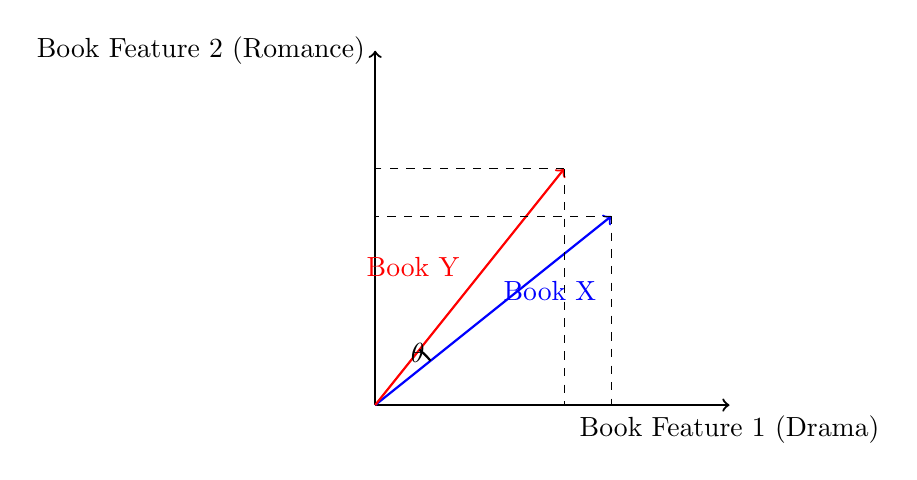
\begin{tikzpicture}[scale=3]

% Axes
\draw[->, thick] (0,0) -- (1.5,0) node[anchor=north] {Book Feature 1 (Drama)};
\draw[->, thick] (0,0) -- (0,1.5) node[anchor=east] {Book Feature 2 (Romance)};

% Define vectors
\coordinate (X) at (1,0.8);
\coordinate (Y) at (0.8,1);

% Draw book vectors
\draw[->, thick, blue] (0,0) -- (X) node[midway, above right] {Book X};
\draw[->, thick, red] (0,0) -- (Y) node[midway, above left] {Book Y};

% Dashed projections to axes for Book X
\draw[dashed] (X) -- (X|-0,0); % to x-axis
\draw[dashed] (X) -- (0,0|-X); % to y-axis

% Dashed projections to axes for Book Y
\draw[dashed] (Y) -- (Y|-0,0); % to x-axis
\draw[dashed] (Y) -- (0,0|-Y); % to y-axis

% Compute angles of vectors
\pgfmathsetmacro{\angleX}{atan2(0.8,1)} % vector X
\pgfmathsetmacro{\angleY}{atan2(1,0.8)} % vector Y

% Draw angle arc between vectors
\draw[thick] (0,0) +(\angleX:0.3) arc[start angle=\angleX, end angle=\angleY, radius=0.3];
\node at (0.18,0.22) {$\theta$};

\end{tikzpicture}


Here, $\theta$ is the angle between vectors $\mathbf{x}$ and $\mathbf{y}$. Cosine similarity measures how aligned these vectors are: the smaller the angle, the closer the similarity is to 1.

\textbf{Intuition:} Cosine similarity focuses on the direction of vectors rather than their magnitude. Two items with similar feature patterns
 are considered similar, even if one has generally higher values than the other.

The formula for cosine similarity between two item vectors $\mathbf{x}$ and $\mathbf{y}$ is:

\begin{equation}
\text{sim}(\mathbf{x}, \mathbf{y}) = \frac{\mathbf{x} \cdot \mathbf{y}}{\|\mathbf{x}\| \, \|\mathbf{y}\|} 
= \frac{\sum_{i=1}^{n} x_i y_i}{\sqrt{\sum_{i=1}^{n} x_i^2} \; \sqrt{\sum_{i=1}^{n} y_i^2}}
\end{equation}

Here, $\mathbf{x} \cdot \mathbf{y}$ represents the dot product of the two vectors, where $\mathbf{x}$ and $\mathbf{y}$ are vectors, for example,
item feature vectors in a recommendation system and $\|\mathbf{x}\|$ and $\|\mathbf{y}\|$ are the magnitudes (lengths) of the vectors.
This metric allows the system to quantify similarity between items and recommend those that are most closely aligned with the user's
previous preferences.

In content-based filtering, each item is represented as a vector in a multi-dimensional feature space. For example, a book could be represented as
\[
\mathbf{x} = [\text{drama score}, \text{romance score}, \text{adventure score}, \dots].
\]

\begin{itemize}
    \item The \textbf{dot product} of two vectors $\mathbf{x}$ and $\mathbf{y}$ quantifies how much the vectors point in the same direction:
    \[
    \mathbf{x} \cdot \mathbf{y} = x_1 y_1 + x_2 y_2 + \dots + x_n y_n = \sum_{i=1}^{n} x_i y_i
    \]
    Each term represents the contribution of a feature to the overall similarity.
    \item The \textbf{norm} or length of a vector is:
    \[
    \|\mathbf{x}\| = \sqrt{x_1^2 + x_2^2 + \dots + x_n^2}
    \]
    Normalizing by the vector lengths ensures that cosine similarity measures direction rather than magnitude.
\end{itemize}

Cosine similarity is then defined as:
\[
\text{sim}(\mathbf{x}, \mathbf{y}) = \frac{\mathbf{x} \cdot \mathbf{y}}{\|\mathbf{x}\| \, \|\mathbf{y}\|} = \cos \theta
\]

\noindent where $\theta$ is the angle between the vectors. The similarity ranges from $-1$ (opposite) to $1$ (identical), with $0$ indicating orthogonal (no similarity).

\subsubsection{Euclidean Distance}

Euclidean distance is a way to measure how far apart two items are in a multi-dimensional feature space. It is the length of the straight line connecting the two points representing the items. In recommendation systems, a smaller Euclidean distance between two items indicates that they are more similar in terms of their features.

Suppose we represent two books as feature vectors:
\[
\mathbf{x} = (\text{drama score}, \text{romance score}, \dots), \quad
\mathbf{y} = (\text{drama score}, \text{romance score}, \dots)
\]

For \(n\) features, the Euclidean distance between \(\mathbf{x}\) and \(\mathbf{y}\) is:

\begin{equation}
d(\mathbf{x}, \mathbf{y}) = \sqrt{ (\text{drama}_x - \text{drama}_y)^2 + (\text{romance}_x - \text{romance}_y)^2 + \dots }
= \sqrt{ \sum_{i=1}^{n} (x_i - y_i)^2 }
\end{equation}

\begin{itemize}
    \item Each term \((x_i - y_i)^2\) measures the squared difference in a single feature (e.g., drama, romance) between the two books.
    \item Summing over all features gives a combined measure of difference across all dimensions.
    \item Taking the square root converts this sum into the actual straight-line distance.
\end{itemize}

\textbf{Intuition:}  
- Two books with similar ratings across all features will have a **small Euclidean distance**.  
- Books with very different ratings in one or more features will have a **larger distance**.  

\medskip

\begin{center}
\begin{tikzpicture}[scale=2]

% Axes
\draw[->, thick] (0,0) -- (4,0) node[right] {Drama};
\draw[->, thick] (0,0) -- (0,4) node[above] {Romance};

% Points representing books
\coordinate (X) at (1.5,2.5);
\coordinate (Y) at (3,1);

% Draw points
\filldraw[blue] (X) circle (2pt) node[above left] {Book X};
\filldraw[red] (Y) circle (2pt) node[below right] {Book Y};

% Draw Euclidean distance
\draw[dashed, thick] (X) -- (Y) node[midway, above, sloped] {$d(\mathbf{x},\mathbf{y})$};

% Dotted projections for Book X
\draw[dotted, gray] (X) -- (X|-0,0); % horizontal to x-axis
\draw[dotted, gray] (X) -- (0,0|-X); % vertical to y-axis

% Dotted projections for Book Y
\draw[dotted, gray] (Y) -- (Y|-0,0); % horizontal to x-axis
\draw[dotted, gray] (Y) -- (0,0|-Y); % vertical to y-axis

\end{tikzpicture}
\end{center}


This diagram shows:
\begin{itemize}
    \item Each book as a point in a 2D feature space (Drama vs Romance).  
    \item The dashed line representing the Euclidean distance between the books.  
    \item Dotted lines showing the projections to each feature axis for clarity.  
\end{itemize}


\subsection{Pearson Correlation}\label{sec:pearson}

Pearson correlation measures the **linear relationship** between two items across multiple features. Unlike cosine similarity or Euclidean distance, Pearson correlation **removes the effect of magnitude** by centering each vector on its mean. This makes it useful when we care about **rating patterns** rather than absolute values.

\paragraph{Definition}

Given two books represented as feature vectors:
\[
\mathbf{x} = [\text{drama}_x, \text{romance}_x, \dots], \quad
\mathbf{y} = [\text{drama}_y, \text{romance}_y, \dots]
\]

Let \(\bar{x}\) and \(\bar{y}\) be the mean values of the features of each book:
\[
\bar{x} = \frac{1}{n} \sum_{i=1}^{n} x_i, \quad
\bar{y} = \frac{1}{n} \sum_{i=1}^{n} y_i
\]

The Pearson correlation is:

\begin{equation}
\text{corr}(\mathbf{x}, \mathbf{y}) =
\frac{\sum_{i=1}^{n} (x_i - \bar{x}) (y_i - \bar{y})}
     {\sqrt{\sum_{i=1}^{n} (x_i - \bar{x})^2} \; \sqrt{\sum_{i=1}^{n} (y_i - \bar{y})^2}}
\end{equation}

\begin{itemize}
    \item Each feature is **mean-centered**: we subtract the book's average feature value.  
    \item The numerator computes the **covariance** between the two books' features.  
    \item The denominator normalizes by the magnitude of the mean-centered vectors, giving a value between \(-1\) and \(1\).  
\end{itemize}

\paragraph{Interpretation}

\begin{itemize}
    \item \(+1\) → features vary together perfectly (strong positive correlation).  
    \item \(0\) → no linear relationship between features.  
    \item \(-1\) → features vary in opposite directions (strong negative correlation).  
\end{itemize}

\medskip

\textbf{Example in 2D feature space: Drama vs Romance}

\begin{center}
\begin{tikzpicture}[scale=2]

% Axes
\draw[->, thick] (0,0) -- (4,0) node[right] {Drama};
\draw[->, thick] (0,0) -- (0,4) node[above] {Romance};

% Original book vectors
\coordinate (X) at (1.5,2.5);
\coordinate (Y) at (3,1);

% Draw points
\filldraw[blue] (X) circle (2pt) node[above left] {Book X};
\filldraw[red] (Y) circle (2pt) node[below right] {Book Y};

% Mean-centered vectors (shifted to origin)
\coordinate (Xc) at (X);
\coordinate (Yc) at (Y);

% Draw dashed line connecting mean-centered vectors
\draw[dashed, thick] (Xc) -- (Yc) node[midway, above, sloped] {covariance component};

% Draw axes from mean
\draw[dotted, gray] (Xc) -- (Xc|-0,0); % horizontal projection
\draw[dotted, gray] (Xc) -- (0,0|-Xc); % vertical projection
\draw[dotted, gray] (Yc) -- (Yc|-0,0); % horizontal projection
\draw[dotted, gray] (Yc) -- (0,0|-Yc); % vertical projection

\end{tikzpicture}
\end{center}

\textbf{Notes:}  
\begin{itemize}
    \item The vectors are **mean-centered** by subtracting each book's average feature value.  
    \item The dashed line visually represents the **co-movement of features** contributing to Pearson correlation.  
    \item This method measures **pattern similarity**, so two books with similar relative features but different absolute levels can still have a high correlation.
\end{itemize}

